\documentclass[10pt]{article}

\usepackage[T1]{fontenc}
\usepackage{geometry}
\usepackage{amsmath, amssymb, amsthm}
\usepackage{array} 
\usepackage{enumitem}
\usepackage{siunitx}
\usepackage{graphicx}
% \usepackage{caption}
\usepackage{chemformula}

\geometry{a4paper, margin=1in}
\setlength\parindent{0pt}
% \renewcommand\qedsymbol{$\blacksquare$}
\newcolumntype{L}{l@{\quad\quad}}
\newcounter{prob}
\def\problem{\stepcounter{prob}\paragraph{Problem \arabic{prob}}}
\def\solution{\\\\\textbf{Solution }}

\begin{document}
        \par\textbf{IISER Kolkata} \hfill \textbf{Assignment VI}
        \vspace{3pt}
        \hrule
        \vspace{3pt}
        \begin{center}
                \LARGE{\textbf{CH1201 : General Physical Chemistry}}
        \end{center}
        \vspace{3pt}
        \hrule
        \vspace{3pt}
        Satvik Saha, \texttt{19MS154}\hfill\today
        \vspace{20pt}

        \textit{Note:} All logarithms are natural unless specified otherwise.

        \problem Is the activation energy $E_a$ dependent on temperature? Qualitatively draw an $E_a$ versus temperature plot, i.e.\ 
        represent how $E_a$ changes with reaction temperature.
        \solution The activation energy represents the extra energy required by reactant molecules to reach an `activated complex',
        a state where the formation and breaking of bonds along with restructuring of the molecule takes place. Thus, it is the 
        difference between the energy of such an activated complex $E_X$ and the average energy of the reactant molecules $E_A$. \\
        
        The activation energy for the forward reaction $E_{a,1}$ is thus given by $E_X - E_A$, and that of the backward reaction
        $E_{a,-1}$ is given by $E_X - E_B$, where $E_B$ is the average energy of the products. The heat of 
        the reaction $\Delta H = E_B - E_A = E_{a,1} - E_{a,-1}$ is given by the Van't Hoff equation
        \[
        \frac{\mathrm{d}\log{K}}{\mathrm{d}{T}} \;=\; \frac{\Delta{H}}{RT^2}.
        \]
        Here, the equilibrium constant $K = k /k_{-1}$ is the ratio of the rate constants for the forward and backward reaactions.
        Separating the forward reaction, we have the relation
        \[
        E_a \;=\; RT^2\, \frac{\mathrm{d}\log{k}}{\mathrm{d}{T}}.
        \]
        Integration and rearrangement yields the Arrhenius equation $k = Ae^{-E_a / RT}$, or
        \[
        \log{k} \;=\; -\frac{E_a}{RT} + \log{A}.
        \]

        Another approach is to interpret $E_a$ in terms of the Gibbs energy of activation, given by the relations
        $\Delta G^\ddagger = -RT\log{k} = \Delta H^\ddagger - T\Delta S^\ddagger$, where $\Delta H^\ddagger$ is the enthalpy of activation
        and $\Delta S^\ddagger$ is the entropy of activation for the forward reaction. Rearranging, we obtain the Eyring equation
        \[
        \log{k} \;=\; -\frac{\Delta H^\ddagger}{RT} + \frac{\Delta S^\ddagger}{R}.
        \]
        Comparing this with the Arrhenius equation gives $E_a = \Delta H^\ddagger + RT$. \\

        For typical reaction temperatures, the activation energy $E_a$ is assumed to be independent of temperature.
        Empirically, a plot of $\log{k}$ vs $1 / T$ is generally a straight line, with constant slope $E_a /R$.
        Although some reactions do not show such a linear trend, this is generally corrected
        by introducing a pre-exponential factor to the Arrhenius equation, such as $k = AT^m e^{-E_a /RT}$ keeping $E_a$ constant.

        \begin{figure}[h!]
        \begin{center}
                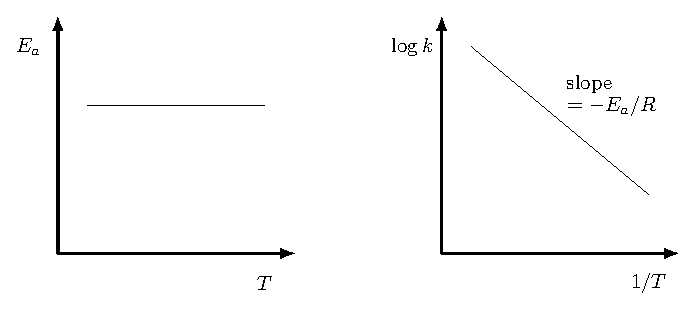
\includegraphics[scale=0.9]{./activation.eps}
        \end{center}
        % \caption*{\it A qualitative description of the activation energy $E_a$.}
        \label{fig:activation}
        \end{figure}

        More precisely, the activation energy of a reaction may be regarded as the minimum amount of energy required in the collision
        between reactant molecules, for the the initiation of the reaction. Increasing the reaction temperature does increase the
        \textit{average kinetic energy} of the reactant, however this does not change the energy threshold, merely the
        \textit{number of molecules} which have that energy. Hence, the impact is purely on the kinetics of the reaction.

        \problem For a chemical reaction, the rate constant at \SI{25}{\celsius} is doubled when the temperature is raised to \SI{45}{\celsius}.
        Determine the activation energy in \SI{}{\kilo\joule\per\mole}.
        \solution We use the Arrhenius equation,
        \[
                k \;=\; Ae^{-E_a /RT}.
        \]
        Considering two different tempereature, $T_1 = \SI{298}{\kelvin}$ and $T_2 = \SI{318}{\kelvin}$, we divide and take logarithms,
        obtaining
        \[
        \log\frac{k_2}{k_1} \;=\; -\frac{E_a}{R} \left[ \frac{1}{T_2} - \frac{1}{T_1} \right].
        \]
        Rearranging, and using $k_2 /k_1 = 2$, we have
        \[
        E_a \;=\; \frac{T_1 T_2}{T_2 - T_1} R \log{2} \;=\; \frac{298\times 318}{318 - 298} \times 8.314 \times \log{2}
                \;=\; \SI{27.3}{\kilo\joule\per\mole}.
        \]

        \problem For a \SI{10}{\celsius} rise in temperature, the rate constant doubles for reaction I and triples for reaction II.
        If both reactions have the same pre-exponential factor, what is the ratio of their activation energies?
        \solution We again use the relation from the previous problem, setting the initial and final temperatures the same for both reactions. Thus,
        \[
        E_a \;\propto\; \log\frac{k_f}{k_i}.
        \]
        Thus, the ratio of activation energies (I over II) is simply $\log{2} /\log{3} \approx 0.631$.

        \problem Explain mathematically how the value of the Michaelis-Menten constant $k_m$ can be obtained for an enzyme catalyzed reaction.
        What factors affect $k_m$?
        \solution Consider a general enzyme catalyzed reaction, with substrate S, enzyme E and products P.
        \[
        \ch{E + S <=>[ k_1 ][ k_2 ] [ES]^* ->[ k_3 ] E + P}
        \]
        Here, [ES]\textsuperscript{*} represents an intermediate complex. Since the amount of enzyme is much less than the amount of substrate,
        we apply a steady state assumption on the intermediate complex, claiming that it's concentration becomes constant over time.
        Thus,
        \[
        \frac{\mathrm{d} [ES]^*}{\mathrm{d}t} \;=\; k_1[E][S] \,-\, k_2 [ES]^* \,-\, k_3[ES]^* \;=\; 0.
        \]
        \[
        [ES]^* \;=\; \frac{k_1}{k_2 + k_3}[E][S].
        \]
        Now, the concentration of the free enzyme can be obtained using conservation as $[E] = [E]_0 - [ES]^*$.
        Plugging this into the relation for [ES]\textsuperscript{*}, and setting $(k_2 + k_3)/ k_1 = k_m$ yields
        \[
        k_m[ES]^* \;=\; ([E]_0 - [ES]^*)[S] \;\implies\; [ES]^* \;=\; \frac{[E]_0 [S]}{k_m + [S]}.
        \]
        The rate of the reaction is governed by the rate of formation of the product, i.e.\ $R \;=\; k_3 [ES]^*$.
        Thus,
        \[
        R \;=\; \frac{k_3 [E]_0 [S]}{k_m + [S]}.
        \]
        This reaches its maximum values when $[S] \gg k_m$, i.e.\ $R_{max} \;=\; k_3 [E]_0$.
        We thus call $k_3$ the turnover rate, i.e.\ the rate of conversion of substrate molecules per molecule of enzyme.\\

        For experimentally determining $k_m$, we use the reciprocal of the previous relation to obtain
        \[
        \frac{1}{R} \;=\; \frac{k_m}{k_3 [E]_0[S]} \,+\, \frac{1}{k_3[E]_0} \;=\; \frac{k_m}{R_{max}} \left( \frac{1}{[S]} \right) \,+\, \frac{1}{R_{max}}.
        \]

        Thus, by varying the concentration of substrate, we obtain a plot of $1 /R$ versus $1 /[S]$ called a Lineweaver-Burk plot.
        Clearly, this has a $y$-intercept of $c = 1 /R_{max}$ and slope $m = k_m/ R_{max}$. The ratio $m /c$ thus yields the Michaelis-Menten
        constant $k_m$. \\

        The factors which affect $k_m$ are pH, temperature, ionic strength and the nature of the substrate.

        \problem How does the Michaelis-Menten equation explain why the rate of an enzyme catalyzed reaction is proportional to the amount of enzyme?
        \solution We use the previously derived Michaelis-Menten equation, 
        \[
        R \;=\; \frac{k_3 [E]_0 [S]}{k_m + [S]}.
        \]
        Note that when the amount of substrate is very large (as it generally is), $R \to k_3 [E]_0$.
        Thus, $R \propto [E]_0$, and is mostly independent of $[S]$.\\

        Essentially, when a large amount of substrate relative to the enzyme is present, the rate of formation of the intermediate
        is limited by the amount of free enzyme present. 
        Note that the total amount of enzyme (free or bound in the intermediate complex) is conserved.
        Thus, the rate of formation of the product, which is directly proportional to the 
        amount of intermediate, is also proportional to the amount of enzyme supplied.

        \problem For an enzyme catalyzed reaction, the Lineweaver-Burk plot resulted in a slope and intercept values of \SI{3.5e-2}{\s}
        and \SI{5e4}{\per\mole\litre\s} respectively. Estimate $k_m$ and the turnover number when the initial concentration
        of the enzyme is \SI{2.5e-9}{\mole\per\litre}.
        \solution We simply use $k_m = \text{slope}/\text{intercept}$ to obtain 
        \[
        k_m \;=\; \frac{3.5 \times 10^{-2}}{5\times 10^4} \;=\; \SI{7e-7}{\mole\per\litre}.
        \]
        Note that the intercept is simply $1 /R_{max}$.
        Now, the turnover number $k_3$ is given by
        \[
        k_3 \;=\; \frac{R_{max}}{[E]_0} \;=\;  \frac{1}{5\times 10^4 \times 2.5\times 10^{-9}} \;=\; \SI{8000}{\per\s}.
        \]

        \problem In the Lindemann mechanism of unimolecular reactions, what is the observed order at low concentration?
        \solution The Lindemann mechanism posits the following steps.
        \[
        \ch{ A + A <=>[ k_1 ][ k_2 ] A + A^*}
        \]
        \[
        \ch{A^* ->[ k_3 ] P}
        \]
        Here, A\textsuperscript{*} is the activated reactant and P is the decomposition product(s).
        Since activatd molecules are short lived, we impose a steady state condition on them.
        \[
        \frac{\mathrm{d} [A^*]}{\mathrm{d}t} \;=\; k_1 [A]^2 \,-\, k_2[A][A^*] \,-\, k_3[A^*] \;=\; 0.
        \]
        \[
        [A^*] \;=\; \frac{k_1 [A]^2}{k_3 + k_2[A]}.
        \]
        The rate of the reaction is again governed by the formation of the product, i.e.\ $R = k_3[A^*]$. Hence,
        \[
        R \;=\; \frac{k_1k_3[A]^2}{k_3 + k_2[A]}.
        \]
        Now, when $[A]$ is very low, we make the approximation $k_3 \gg k_2[A]$. This means that the rate of deactivation
        is very low, because of fewer collisions. Thus, the denominator in the rate law tends to $k_3$, giving
        $R = k_1 [A]^2$. This behaviour is second order with respect to the concentration of the reactant $[A]$.

        \problem Give the kinetics of the thermal decomposition of \ch{CH_3CHO}.
        \solution We propose that the thermal decomposition of \ch{CH_3CHO} takes place via a chain reaction.
        \[
        \ch{CH_3CHO ->[ $\Delta$ ] CH_4 + CO}
        \]
        The initiation and propagation steps involve the synthesis of intermediate radicals.
        \begin{align*}
                \ch{
                        CH_3CHO                 &->[ k_1 ] ^.CH_3 + ^.CHO  \\
                        CH_3CHO + ^.CH_3        &->[ k_2 ] CH_4 + CH_3CO^. \\
                        CH_3CO^.                &->[ k_3 ] ^.CH_3 + CO \\
                        ^.CH_3 + ^.CH_3         &->[ k_4 ] C_2H_6
                }
        \end{align*}
        Applying the steady state assumption on the intermediates,
        \[
        \frac{\mathrm{d} [\ch{^.CH_3}]}{\mathrm{d}t} \;=\; k_1[\ch{CH_3CHO}] - k_2[\ch{CH_3CHO}][\ch{^.CH_3}] + k_3[\ch{CH_3CO^.}] - 2k_4[\ch{^.CH_3}]^2 = 0
        \]
        \[
        \frac{\mathrm{d} [\ch{CH_3CO^.}]}{\mathrm{d}t} \;=\; k_2[\ch{CH_3CHO}][\ch{^.CH_3}] - k_3[\ch{CH_3CO^.}] = 0
        \]
        Adding these together,
        \[
        k_1[\ch{CH_3CHO}] \;=\; 2k_4[\ch{^.CH_3}]^2 \quad\implies\quad [\ch{^.CH_3}] \;=\; \sqrt{\frac{k_1}{2k_4}\ch{[CH_3CHO}]}.
        \]
        Hence, the rate of the reaction is given by the rate of formation of methane, i.e.\ 
        \[
                R \;=\; \frac{\mathrm{d} [\ch{CH_4}]}{\mathrm{d}t} \;=\; k_2[\ch{CH_3CHO}][\ch{^.CH_3}] \;=\; 
                        \sqrt{\frac{k_2^2k_1}{2k_4}}[\ch{CH_3CHO}]^{3 / 2}.
        \]
        Thus, the rate of the reaction is of $3 /2$ order with respect to the concentration of acetaldehyde.

        \problem On irradiation of propionaldehyde at \SI{30}{\celsius} with light of wavelength \SI{3020}{\angstrom}, the quantum yield
        for the production of \ch{CO} is observed to be $0.54$. If the incident light intensity is \SI{15000}{erg\per\s},
        calculate the rate of \ch{CO} formation. What is the light intensity in Einstein per second?
        \solution A wavelength of \SI{3020}{\angstrom} corresponds to an energy of $E = hc/\lambda = \SI{6.58e-19}{\joule}$
        per photon. Now, using 1 erg = $10^{-7}$\SI{}{\joule}, the given light intensity is $I = \SI{1.5e-3}{\joule\per\s}$.
        This corresponds to $n = I / E = \SI{2.28e15}{}$ photons per second, i.e.\ $N = n / N_A = \SI{3.79e-9}{\mole}$ photons per second.
        Thus, the rate of production of \ch{CO} is simply $\phi n = \SI{1.23e15}{}$ molecules per second, or $\phi N = \SI{2.04e-9}{\mole\per\s}$. \\

        The energy of \SI{1}{\mol} of photons here is $N_AE = \SI{3.96e5}{\joule}$. Thus, the given light intensity corresponds to
        $I /(N_A E) = \SI{3.79e-9}{Einstein\per\s}$.

\end{document}
